\chapter{Improvement of entropic criteria} \label{chap:criteria}

\section{Bounds based on meet}

\subsection{Separability criterion}

The second result of this master thesis is to improve some entropic criteria tied to majorization relations. As stated in theorem \ref{th:majorization_separability_criterion}, if a bipartite state $\rho^{AB}$ is separable, then

\begin{equation}
    \lambda^{AB} \prec \lambda^A \quad \text{and} \quad \lambda^{AB} \prec \lambda^{B},
\end{equation}

where $\lambda^X$ is the ordered vector of eigenvalues of the density matrix of system $X$. By Schur-concavity of $H$, this directly implies

\begin{equation}
    H(\lambda^{AB}) \geq H(\lambda^A) \quad \text{and} \quad H(\lambda^{AB}) \geq H(\lambda^B).
\end{equation}

These entropic inequalities\footnote{Historically, these entropic inequalities (expressed equivalently in von Neumann entropies) were known before the strengthening to a majorization relation \cite{cerf_negative_1997, nielsen_separable_2001}.} are of course not as strong as the majorization relations we deduced them from, as illustrated in the example from section \ref{sec:majorization_separability_criterion}. Using the lattice, however, the entropic condition can be strengthened. The relations $\lambda^{AB} \prec \lambda^A$ and $\lambda^{AB} \prec \lambda^{B}$ mean that $\lambda^{AB}$ is majorized by both $\lambda^A$ and $\lambda^B$. By definition, the meet of $\lambda^A$ and $\lambda^B$ is the vector $\lambda^A \wedge \lambda^B$ that majorizes all the vectors that are majorized by both $\lambda^A$ and $\lambda^B$. This fact can also be restated as 

\begin{equation}
    \mathcal{T}_-(\lambda^A) \cap \mathcal{T}_-(\lambda^B) = \mathcal{T}_-(\lambda^A \wedge \lambda^B),
\end{equation}

\noindent using definition \ref{def:majorization_cones} of majorization cones. Applying this to the separability criterion, we get that if $\rho^{AB}$ is a separable state, then

\begin{equation}
    \lambda^{AB} \prec \lambda^A \; \text{and} \; \lambda^{AB} \prec \lambda^{B} \; \iff \; \lambda^{AB} \prec \lambda^A \wedge \lambda^B \; \implies \; H(\lambda^{AB}) \geq H(\lambda^A \wedge \lambda^B).
\end{equation}

This new formulation in terms of entropies is a strengthening of the initial entropic criterion, providing a better lower bound on the entropy of a separable state. However, it is still not as strong as the majorization criterion itself. Moreover, this new entropic criterion based on the meet is not very interesting for pure bipartite states because of corollary \ref{cor:reduced_schmidt}, which essentially states that $\lambda^A = \lambda^B$ if $\rho^{AB}$ is pure. In that case $\lambda^A \wedge \lambda^B = \lambda^A = \lambda^B$, and the new entropic criterion reduces to the original one. Unfortunately, pure bipartite states are the more interesting states for quantum computation: decoherence (i.e. losing purity by interacting with the environment) is never a desired feature for qubits as mixed states introduce uncertainty into computations, causing them to fail with a certain probability. Figure \ref{fig:improved_criterion} illustrates the new criterion.

\begin{figure}[h!]
    \centering
    \begin{tikzpicture}[scale=0.9]
        % draw cone of p
        \coordinate (A) at (-2, 3);
        \coordinate (B) at (1, -1.5);
        \draw[dotted] [name path=A--B, color=gray] (A) -- (B);
        \coordinate (C) at (-1,-1.5);
        \coordinate (D) at (2,3);
        \draw[dotted] [name path=C--D, color=gray] (C) -- (D);
        \path [name intersections={of=A--B and C--D,by=E}];
        \node [fill=black,inner sep=1pt,label=180:$\lambda^A$] at (E) {};
        % draw cone of q
        \coordinate (F) at (-0.166,3);
        \coordinate (G) at (2.833, -1.5);
        \draw[dotted] [name path=F--G, color=gray] (F) -- (G);
        \coordinate (H) at (2.166,-1.5);
        \coordinate (I) at (4.966,3);
        \draw[dotted] [name path=H--I, color=gray] (H) -- (I);
        \path [name intersections={of=F--G and H--I,by=J}];
        \node [fill=black,inner sep=1pt,label=0:$\lambda^B$] at (J) {};
        %intersections of the 2 cones
        \path [name intersections={of=F--G and C--D,by=K}];
        %\path [name intersections={of=H--I and A--B,by=L}];
        \node [fill=black,inner sep=1pt,label=90:$\lambda^A \wedge \lambda^B$] at (K) {};
        %\node [fill=black,inner sep=1pt] at (L) {};
        %\node [inner sep=4pt, label=270:$p \vee q$] at (L) {}; % virtual point to set the label further away (otherwise the fill gets bigger too)
        % create the entropy arrow
        \coordinate (M) at (-3, -1.5);
        \coordinate (N) at (-3, 3);
        \coordinate (N') at (-3, 3.3);
        \coordinate (O) at (5, 1.33);
        \coordinate (P) at (5, 3);
        \coordinate (Q) at (5, -1.5);
        \coordinate (R) at (-3, 1.33);
        \coordinate (S) at (-3.5, 1.33);

        \draw[->] (M) -- (N');
        \node [inner sep=0pt, label=180:$H(\lambda^{AB})$] at (N') {};
        \draw[dotted] [name path=old_left, color=gray] (E) -| (M);
        \draw[dotted] [name path=old_right, color=gray] (E) -| (5,0);
        \draw[dotted] [name path=new_left, color=gray] (K) -| (S);
        \draw[dotted] [name path=new_right, color=gray] (K) -| (O);
        % fill the 2 zones for the criterion
        \fill[fill=blue, opacity=0.15] (N) -- (R) -- (O) -- (P) -- cycle;
        \fill[fill=red, opacity=0.15] (M) -- (R) -- (O) -- (Q) -- cycle;
        \node [inner sep=3pt, label=135:{Maybe entangled, maybe separable}] at (R) {};
        \node [inner sep=3pt, label=225:{Entangled}] at (R) {};

    \end{tikzpicture}
    \caption{Depiction of the improved entropic criterion for entanglement. The previous criterion could not decide whether states with $\lambda^{AB}$ with an entropy between the two horizontal doted lines going through $\lambda^A$ and $\lambda^A \wedge \lambda^B$ were entangled. The new criterion shows that they are.}
    \label{fig:improved_criterion}
\end{figure}

Another important caveat to this criterion is that if $\lambda^A \sim \lambda^B$, then $\lambda^A \wedge \lambda^B = \lambda^A$ or $\lambda^B$ (whichever is majorized by the other), and the criterion reduces to the original one. As such, it seems that something interesting is happening when two vectors are incomparable, as incomparability enables us to improve entropic criteria. This very notion, of quantifying the amount of incomparability between two probability vectors and considering it a resource, is the idea that led to chapter \ref{chap:incomparability}.


This means that our criterion is \textit{a priori} not particularly useful in the context of quantum information, however it could still be useful in experiments trying to assert whether a state is entangled or not. In such cases, the majorization relations can be hard to use because the vector of eigenvalues of the density operator can be hard to determine experimentally. However, the measurement statistics can be used to compute the Shannon entropy of the distributions easily. As such, if one could experimentally construct a state with the same eigenvalues as $\lambda^A \wedge \lambda^B$, one could measure its statistics and use the better lower bound to determine whether the joint state is separable. Unfortunately, no obvious way to construct this state, which we will note $\rho_{A \wedge B}$, was found. For example, constructing this state with an interferometer in quantum optics would require the construction of the meet (cf. section \ref{sec:meet}) to have a known formulation in terms of unitary operators. An additional constraint is that the action of an interferometer cannot decrease the entropy of a state CITATION NEEDED, which means that the subadditivity property of Shannon entropy (cf. theorem \ref{th:shannon_subadditivity}) prevents us from constructing an interferometer that only outputs the meet of two entry states because

\begin{equation}
    H(\rho_{A \wedge B}) \leq H(\rho_A) + H(\rho_B).
\end{equation}

However, an interferometer outputting both $\rho_{A \wedge B}$ and a state with the same eigenvalues as $\lambda^A \vee \lambda^B$, which we will call $\rho_{A \vee B}$, does not violate this entropic principle because thanks to supermodularity (cf. theorem \ref{th:shannon_supermodularity})

\begin{equation}
    H(\rho_{A \wedge B}) + H(\rho_{A \vee B}) \geq H(\rho_A) + H(\rho_B),
\end{equation}

\noindent and so the entropy increases after traversing the interferometer. However, even if the interferometer outputs both states, nothing forces us to use $\rho_{A \vee B}$ for any measurements, and so we can still use $\rho_{A \wedge B}$ for the improved entropic criterion.

We suspect that such an interferometer might be possible, but no clear lead on designing the interferometer has been found because it is not clear how the meet and join constructions might be possible with unitaries. We have

\begin{align}
    a_i &= \min \Big\{ \sum_{j=1}^{i} p_j , \sum_{j=1}^{i} q_j \Big\} - \sum_{j=1}^{i-1} a_j\\
    &= \min \Big\{ \sum_{j=1}^{i} p_j , \sum_{j=1}^{i} q_j \Big\} - \min \Big\{ \sum_{j=1}^{i-1} p_j , \sum_{j=1}^{i-1} q_j \Big\}\\
    b_i &= \max \Big\{ \sum_{j=1}^{i} p_j , \sum_{j=1}^{i} q_j \Big\} - \sum_{j=1}^{i-1} b_j\\
    &= \max \Big\{ \sum_{j=1}^{i} p_j , \sum_{j=1}^{i} q_j \Big\} - \max \Big\{ \sum_{j=1}^{i-1} p_j , \sum_{j=1}^{i-1} q_j \Big\},
\end{align}

\noindent where we use $\beta(p, q)$ instead of the true join because the smoothing algorithm is an additional layer of complexity (and is not needed to satisfy the increase in entropy). The minima and maxima of those expressions seem difficult to realize with unitaries. However, we suspect that nonlinear devices might help in achieving such behavior CITATION NEEDED.

% enft ecrire ca comme ca me donne des idees lol, peut-etre pas impossible enft

\subsection{Other criteria}

The previous discussion is not unique to quantum information and separability. Any other branch of physics working with coupled majorization relations but struggling to use them in practice might benefit from constructing the equivalent of a state $\rho_{A \wedge B}$ and computing the entropy of the resulting distribution. For example, another field that deals with majorization relations is the field of quantum thermodynamics, where allowed state transformations under thermal operations are bound to thermomajorization cones (called thermal cones), analogously to entanglement cones in LOCC \cite{junior_geometric_2022, korzekwa_structure_2017}. On the flip-side, this kind of entropic criterion based on the meet could also be used as an experimental sign\footnote{Not evidence, however, as the improved entropic criterion is still weaker than the majorization relation.} of an underlying majorization relation, in cases where one suspects that there is something deeper going on than only the entropic inequalities.



\section{Numerical simulations}

\subsection{Renyi entropies}

The improved criterion is not unique to Shannon entropy. All Rényi entropies $H_\alpha$ are Schur-concave, and so
\begin{align}
    \lambda^{AB} \prec \lambda^A \; \text{and} \; \lambda^{AB} \prec \lambda^{B} \; &\iff \; \lambda^{AB} \prec \lambda^A \wedge \lambda^B \;\\ &\implies \; H_\alpha(\lambda^{AB}) \geq H_\alpha(\lambda^A \wedge \lambda^B) \quad \forall \alpha \in \mathbb{R}^+.
\end{align}

A numerical analysis was carried out to figure out whether there exists an optimal $\alpha$ for which the improved criterion triggers the most amount of times, relative to the original criterion. This was simulated in the context of entanglement by generating random density matrices using QuTip with a specified tensor structure until the majorization criterion $\lambda^A \wedge \lambda^B \prec \lambda^{AB}$ is met. This way, 10000 strongly entangled states are generated. Then, the Rényi-entropic criterion was used on each of these strongly entangled states by iterating over the value of $\alpha$, with a step of 0.2, and each entanglement detection was recorded. Finally, this process is repeated for several dimensions of interest. An implementation of this test is available on the \href{https://github.com/traaldbjerg/MajoLat}{GitHub for the project}.

Computationally, the eigenvalue calculations of the operators and reduced operators become very heavy as the dimensions increase, so the largest dimensions attempted were 3 by 6 before the computation time became prohibitive. The 2 by 2 case is not shown because incomparability is not possible in two dimensions and so the meet criterion reduces to the old one. The final results are shown in figures \ref{fig:renyi_comparison}.

\begin{figure}[ht] 
  \begin{subfigure}[b]{0.5\linewidth}
    \centering
    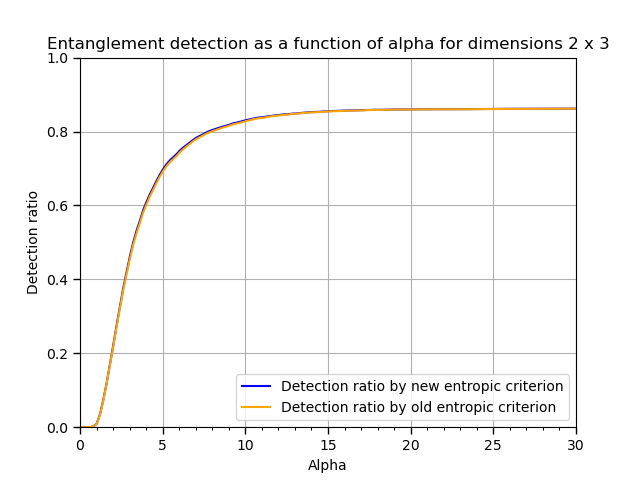
\includegraphics[width=\linewidth]{images/renyi_comparison_2_3_30_0.2.png} 
    \caption{Entanglement detection ratios as a function of $\alpha$ for dimensions 2 $\times$ 3.} 
    \label{fig:renyi_2x3} 
    \vspace{2ex}
  \end{subfigure}%% 
  \begin{subfigure}[b]{0.5\linewidth}
    \centering
    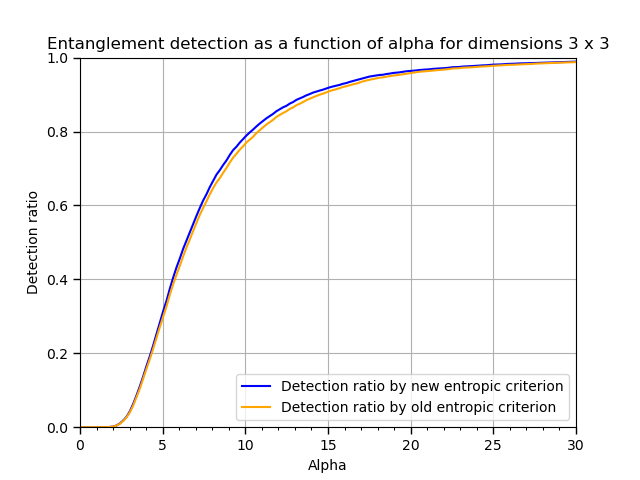
\includegraphics[width=\linewidth]{images/renyi_comparison_3_3_30_0.2.png} 
    \caption{Entanglement detection ratios as a function of $\alpha$ for dimensions 3 $\times$ 3.} 
    \label{fig:renyi_3x3} 
    \vspace{2ex}
  \end{subfigure} 
  \begin{subfigure}[b]{0.5\linewidth}
    \centering
    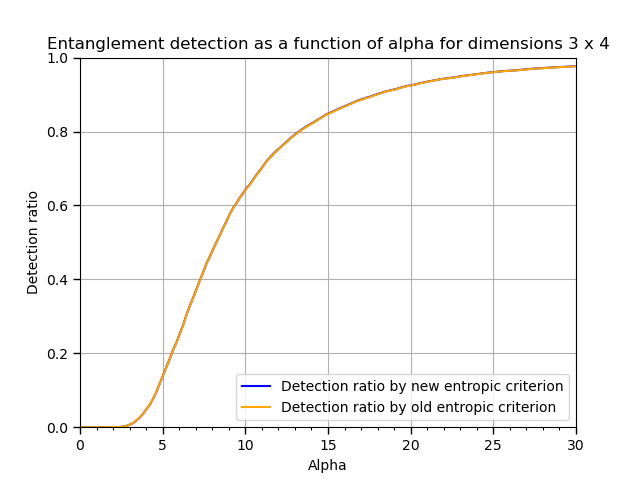
\includegraphics[width=\linewidth]{images/renyi_comparison_3_4_30_0.2.png} 
    \caption{Entanglement detection ratios as a function of $\alpha$ for dimensions 3 $\times$ 4.} 
    \label{fig:renyi_3x4} 
  \end{subfigure}%%
  \begin{subfigure}[b]{0.5\linewidth}
    \centering
    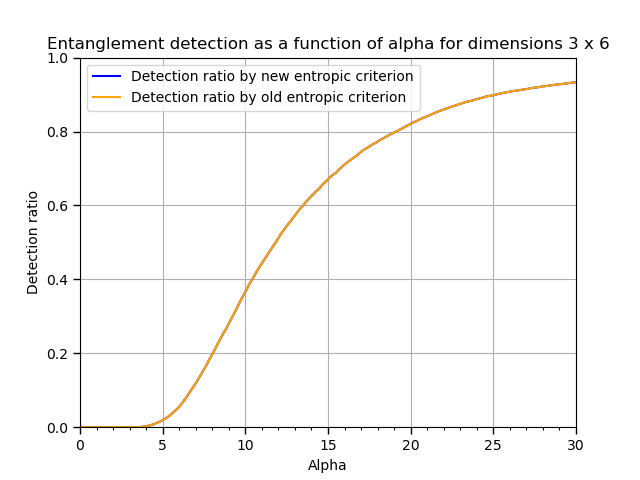
\includegraphics[width=\linewidth]{images/renyi_comparison_3_6_30_0.2.png} 
    \caption{Entanglement detection ratios as a function of $\alpha$ for dimensions 3 $\times$ 6.} 
    \label{fig:renyi_3x6} 
  \end{subfigure} 
  \caption{Illustration of various images}
  \label{fig:renyi_comparison} 
\end{figure}


\subsection{Discussion}

Interestingly, the Rényi simulation shows that there does seem to be an optimum $\alpha$. Moreover, it seems to be dimension dependent, with a clear optimum in dimension 3 $\times$ 3. Perhaps this hints at some deeper connection between Rényi entropy and majorization, but this research avenue was not explored furter. It is also interesting to note that the improved criterion does not seem to show significant improvements according to the simulation. This might be because of a non-uniform density of quantum states in the $\Delta_{d-1}$ simplex, which might lead to a significant number of random density matrices being drawn close to the bottom of the lattice where the 2 criteria can tell entanglement. Perhas, instead this might be due to reduced states of a density matrix not tending to be too imcomparable from each other, and thus being close to their meet\footnote{This is explained in section \ref{sec:p_monotonicity} with corollary \ref{cor:incomparability_separability}.}. This final idea leads nicely into chapter \ref{chap:incomparability}, where we define and study new objects quantifying the incomparability between probability vectors.